\chapter{A General Introduction of Machine Learning and Machine Translation}
\label{chap:MT}

	\begin{enumerate}
	\item General review of supervised Machine learning \citep{kotsiantis2007supervised}: The goal is provide a high level of understanding of what machine learning is. Machine Learning is to learn from EXAMPLES/SAMPLES. For example, to define the meaning of `dog', instead of giving all the definable features of `dog', we feed the machine with as many as possible of information of entities of dogs that we have access. Montague Semantics is actually a variant of ML, within which `dog' is defined as `the set of all the dog that exists in the current world.'. As such, Montague Semantics is Machine Learning, because instead of defining 'dog' with certain arbitrary rules (+/- FEATURE), it says 'all the dogs entities in the current world'. Definition by samples/examples not by rules.    
	\item Literature on machine translation: from statistical machine translation \citep{koehn2009statistical} to neural machine translation \citep{cho2014learning,cho2014properties,bahdanau2014neural, Koehn_NMT2017}. (Target audience: linguists)
	\end{enumerate}

The current Chapter provides a general literature review and introduction of Machine Learning and Machine Translation, before I report neural net machine translation experiments in Chapter \ref{chap:cake}, \ref{chap:cake2} and \ref{chap:Tying_Up}. The purpose of current Chapter is not meant to be a comprehensive summary of all the technical details of Machine Learning and Machine Translation, but instead this chapter aims to provide high-level descriptions of the algorithms used in Machine Learning and Machine Translation. 

\section{What is Machine Learning?}

This section provides a general, brief and non-technical introduction of Machine Learning.

\subsection{What is a Function and What is a Model?}
Machine learning is a specific algorithm that builds a function. Before we touch upon machine learning, we need to talk about what a function is. Here a function simply means a mapping from an object to another object; to put it in another way, a function takes an input and returns an output. A general form of function is given below:

\begin{exe}
\ex $f: X \rightarrow Y$\\
	or \\
	$ y=f(x) $
\end{exe} 


For example, the following is a simple function that takes a number as input and returns the double of that number:

\begin{exe}
\ex \label{math_function}
\begin{xlist}
\ex $f(x)=2x$
\ex $f: x \rightarrow 2x $\\
	e.g.
	\begin{xlist}
	\ex $f: 1 \rightarrow 2$
	\ex $f: 2 \rightarrow 4$
	\ex $f: 3 \rightarrow 6$
	\ex $\dots$
	\end{xlist}
\end{xlist}
\end{exe}

Grammaticality judgment of a sequence of strings can be viewed as a function, where the input is the sequence and the output is either grammatical or ungrammatical.  

\begin{exe}
\ex 
\begin{xlist}
\ex $English\ Grammar: String \rightarrow Grammaticality$\\
	e.g.
	\begin{xlist}
	\ex $English\ Grammar:  John\ loves\ Mary \rightarrow grammatical $
	\ex $English\ Grammar: loves\ John\ Mary \rightarrow ungrammatical $
	\ex $\dots$
	\end{xlist}
\end{xlist}
\end{exe}

Translation can be viewed as function, too, where the input is a sentence in the source language and the output is a sentence in the target language that conveys the same meaning of the source sentence. For example, a function that translates Scottish Gaelic into English looks like:   

\begin{exe}
\ex 
\begin{xlist}
\ex $Translation_{GaelicToEnglish}: Gaelic\ sentence
 \rightarrow English\ sentence$\\
	e.g.
	\begin{xlist}
	\ex $Translation_{GaelicToEnglish}:\\
	  thuit\ a'\ chlach\ air\ cas\ mo\ mhn`a\\ 
	  \rightarrow\\
	   the\ stone\ fell\ on\ my\ wife's\ foot $
	\ex $Translation_{GaelicToEnglish}:\\
	  tha\ mi\ a'\ sireadh\ an\ leabhair\ bhig\ ghuirm\\
	  \rightarrow\\
	   I\ am\ looking\ for\ the\ small\ blue\ book $
	\ex $\dots$
	\end{xlist}
\end{xlist}
\end{exe}

Expect for mathematical functions like (\ref{math_function}), in most of the cases, we have no direct access to a function. In other words, the function is assumed to be unknown. 
To simulate the behaviors of an unknown function, we build a model with the hope that the model can do the same mapping as the target function.     
Schematically, the relation between a function and a model that simulates that function is depicted below:

\begin{exe}
\ex 
	\begin{xlist}
	\ex \label{fun_dipc} $f: X \rightarrow Y$ (unknown target function)
	\ex \label{model_dipc}$g: X \rightarrow \hat{Y}$ (model)\\
	where $Y \approx \hat{Y}$ 
	\end{xlist}
\end{exe}

(\ref{fun_dipc}) is the unknown target function (conventionally it is represented by $f$ in the literature), and (\ref{model_dipc}) is the model that we build with the hope that it does the same mapping as $f$ (conventionally a model is represented by $g$ in the literature).

In a nutshell, a model is a set of handmade mappings that simulates an unknown function. 

\subsection{Two Different Paradigms of Building a Model}

Now the critical problem is how we build a models to approximate the golden target function. With the unknown target function being the same $f$, there can be two distinctive approaches of building the model: Human-Reasoning Approach and Machine-Learning Approach. 

\begin{exe}
\ex Human-Reasoning Model:
A set of rules manually written by a human that attempts to approximate $f$ based on his or her own knowledge and experiences. 
\end{exe}

The Human-Reasoning approach is built on an individual's knowledge and is task-specific. 
Taking the English grammaticality judgment task as example, this approach will mean that some expert in English grammar will come up a set of rules or some algorithms that can determine whether a sequence of strings is a grammatical English sentences. 
The rules and algorithms are based on this expert's knowledge and they are English specific, and are not applicable to other language.     


Another approach to build a model is using Machine Learning. Instead of building a model from our own reasoning, we may look and all the available examples and come up with a generalization. This is the Machine Learning approach. 
Machine Learning can be defined as follows:

\begin{exe}
\ex Definitions of Machine Learning:
\begin{xlist}
	\ex Machine learning is based on algorithms that can learn from data without relying on rules-based programming \citep{pyle2015executive}. 
	\ex Machine learning algorithms can figure out how to perform important tasks by generalizing from examples \citep{domingos2012few}.
	\ex The field of Machine Learning seeks to answer the question `How can we build computer systems that automatically improve with experience, and what are the fundamental laws that govern all learning processes?' \citep{mitchell2006discipline}.
\end{xlist}
\end{exe}   

For the Machine Learning approach, the most critical factors of how a model is built are 1.) the generic learning algorithms and 2.) the input data from which the generic learning algorithms learns to set up the parameters of the derived model.  

Taking the English grammaticality judgment task as example again, the machine learning approach will first define some generic learning algorithms and then feed the algorithms with labeled sequences, where the label is either `grammatical English sentence' or `ungrammatical English sentence'. Note that the learning algorithms is generic. This means that it is universally applicable. For example, instead of feeding the learning algorithms with English grammaticality label, we may feed the learning algorithms with Scottish Gaelic grammaticality label, and it will able to derive a model that can tell whether a sequence of strings is a grammatical Scottish Gaelic sentence. 


In the genericness and universality of the learning algorithms, there is a reminiscence of Universal Grammar \citep{chomsky2007}. 
Universal Grammar is a type of machine learning. Instead of teaching a set of rules, the children is giving a set of grammatical sentences and then they are able to learn grammar, and produce grammatical sentences. 

\citet{chom2005_three_factors} describes three factors in language design: 1) Universal Grammar, 2) Experience, and 3) other cognitive mechanisms/limitations. This is actually a precise description of how machine learning works. Universal Grammar is the generic learning algorithm. Experience is the training data. Cognitive mechanisms are all the other hardware specification of a machine (i.e. a human brain). So, when the Experience is language X, a child acquires language X.  

  

%\section{A Overview of Theories in Machine Translation}

\section{Statistical Machine Translation}
Statistical Machine Translation uses statistical Machine Learning approaches to build machine translation systems \citep{brown1988statistical, brown1990statistical, brown1993mathematics, koehn2009statistical, moses}. The goal is to build a model that simulates the unknown language mapping function. The training data is parallel corpus, which a collection of pairs of a sentence in one language and the translation of the sentence in another language.

The fundamental translation equation of Statistical Machine Translation is shown as follows:

\begin{equation}
Pr(T|S)=\frac{Pr(T)Pr(S|T)}{Pr(S)}
\end{equation}

In this equation, we try to translate a sentence $S$ in the source language to a sentence $T$ in the target language. The left part of the equation represents the probability of $T$ given $S$. 
The right side of of the equation just flips the conditional probability using Bayes' theorem. 
The advantage of the flipping is that now $Pr(T)$ (the probability of sentence $T$). 
This information can be retrieved by building a language model of the target language, which can estimate the probability of a sequence of strings. $Pr(S|T)$ is the translation model, which measures the probability of $S$ given $T$. 
Given this equation, translating a given sentence $S$ simply means to find a sentence $\hat{T}$ that maximize $Pr(T|S)$.   

\begin{equation}
\hat{T}= \argmax_{T} Pr(T|S) = \argmax_{T} \frac{Pr(T)Pr(S|T)}{Pr(S)} = \argmax_{T} Pr(T)Pr(S|T)
\end{equation}

Now a Statistical Machine Translation system is decomposed into two sub-models: the language model of the target and the translation model. 
To build the language model, the common practice is to train a N-gram model given a corpus. 
To build the translation model, we will need to use parallel corpus. 
To understand the nature of Statistical Machine Translation, we need to look into what information is extracted from the parallel corpus. Critically, the probability of words in the source language aligned with words in the target language is the center of the translation model of Statistical Machine Translation. 

Given how Statistical Machine Translation builds the translation model, Statistical Machine Translation may be viewed as a complicated algorithm of string manipulations and string alignments. 
Importantly, this means that Statistical Machine Translation does not touch upon meaning, which limits the development and performance of Statistical Machine Translation. 

As such, Statistical Machine Translation is doomed to be outperformed by other deeper algorithms that touch upon the domains of meaning. Specifically, 2016 is the year when neural net machine translation started to outperform Statistical Machine Translation. In the Conference on Machine Translation 2016, a neural machine translation system outperformed almost every statistical machine translation systems. And in the following year, the Conference on Machine Translation 2017 went neural. Almost all the submitted papers and models were using neural net machine translation systems. 

In the next section, I will introduce the basics of artificial neural nets and the overview of how neural net machine translation.  

\section{Neural Net Machine Translation}\label{neural_MT}

\subsection{What Is a Artificial Neural Network?}

An artificial neural network is a simple but powerful computation algorithm. It can be viewed as a mathematical function: given an number or a vector of numbers as the input, it will return one and only number or vector. 

Historically, the basic structure of artificial neural networks was long completed more than 60 years ago, as \citet{rosenblatt} described the design and structures of artificial neural networks. 

A simplest neural network is a perceptron. 

\begin{figure}[h]
\caption{Example of a Perceptron \citep{lippmann1987introduction}}
\centering
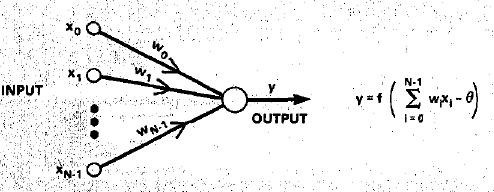
\includegraphics{preceprton.png}
%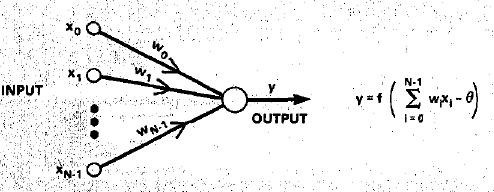
\includegraphics[width=0.5\textwidth]{preceprton.png}
\end{figure}    

\begin{figure}[h]
\caption{A neural network with a hidden layer \citep[p8]{Koehn_NMT2017}}
\centering
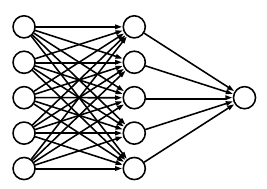
\includegraphics[width=0.5\textwidth]{single_hidden.png}
\end{figure}  


\subsection{Introduction to Neural Net Machine Translation}

\begin{figure}[h]
\caption{Encoder-decoder architecture - example of a general approach for NMT. An encoder converts a source sentence into a "meaning" vector which is passed through a decoder to produce a translation. \citep{luong17GitHub}}
\centering
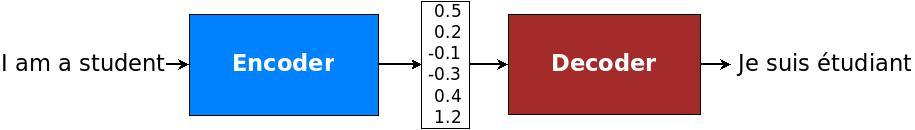
\includegraphics[width=0.9\textwidth]{encdec.jpg}
\end{figure} 


\begin{figure}[h]
\caption{Neural machine translation - example of a deep recurrent architecture proposed by for translating a source sentence ``I am a student" into a target sentence'' "Je suis tudiant". Here, "<s>" marks the start of the decoding process while "</s>" tells the decoder to stop. \citep{luong17GitHub}}
\centering
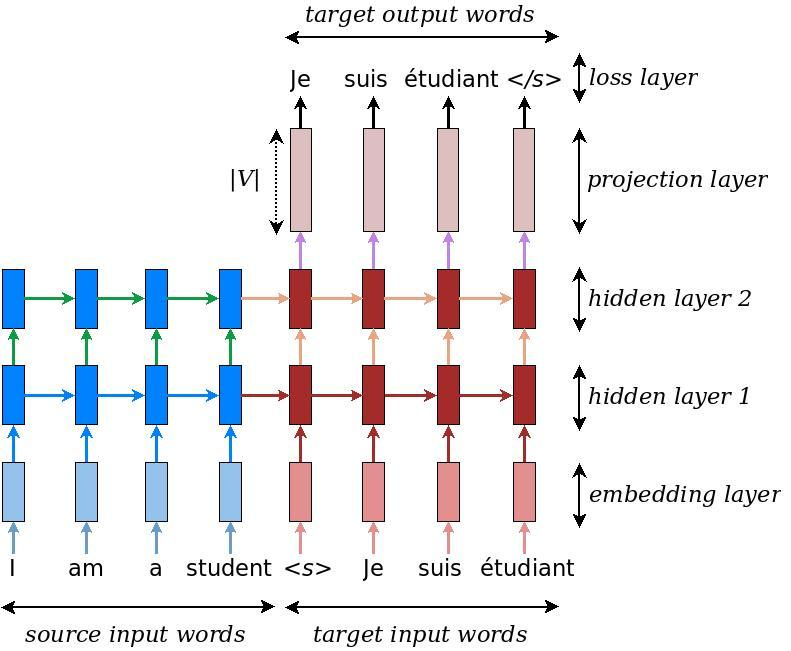
\includegraphics[width=0.9\textwidth]{seq2seq.jpg}
\end{figure} 


\section{A Quick Historical Overview of Machine Translation and Conclusion}

Machine Translation is to automate the process of translating one natural language to another with using computers. The first peak of the developments of Machine Translation started in the 1940s but terminated in 1966. During this period of time, with the advent of the first computers, researchers held high expectations in Machine Translation and lots of resources are shifted into this area. However, in 1966 a report of the Automatic Language Processing Advisory Committee \citep{pierce1966language} terminated this `machine translation rush' as it revealed that too many funds and resources were shifted to Machine Translation without yielding proportional scientific developments. In 1990s, with the advent of Statistical Machine Translation approach developed at IBM, the Machine Translation came back as one of popular scientific areas. Now with the advent of the technique of Artificial Neural Net Machine Learning and other natural language process, Machine Translation is one of the most dynamic research areas.    
